\documentclass{beamer}
\usepackage[utf8]{inputenc}
\usetheme{Antibes}

% À chaque nouvelle section, on dit où on est
\AtBeginSection[ ]
{
 \begin{frame}<beamer>
   \frametitle{Plan}
   \tableofcontents[currentsection]
  \end{frame}
} 

\title{A Dynamic End-to-End Security for Coordinating Multiple Protections within a Linux Desktop}
\subtitle{COLSEC 2010}
\author{J.~Briffaut, M.~Peres \& C. Toinard}
\institute{
\includegraphics[height=1.0cm]{figures/lifo2.png} 
  \hspace{0.5cm} 
\includegraphics[height=1.0cm]{figures/ensib_logo2.png} 
  \hspace{0.5cm} 
\includegraphics[height=1.0cm]{figures/univ_orleans.jpg} 
  \hspace{0.5cm} 
\includegraphics[height=1.0cm]{figures/boken.png}\\
  LIFO, ENSI de Bourges, Université d'Orléans, Boken}

\begin{document}

	% page de garde
	\begin{frame}
		\titlepage
	\end{frame}

	% Ajoute le logo à toutes les autres pages
	\logo{
\includegraphics[height=1.0cm]{figures/ensib_logo.png}}

	\section{Introduction}

		\begin{frame}
			\begin{block}{}
				Today's protection models are:
				\begin{itemize}
					\item mostly static
					\item made of several \& independent security components (firewalls, MAC, etc...)
					\item not adaptating to the user's task
				\end{itemize}
			\end{block}

			\begin{block}{}
				This leads administrators to:
				\begin{itemize}
					\item grant a user all the rights he needs, ever
					\item make use of virtual/physical machines dedicated for every single sensitive task
					\item think about hardware price and usability vs security
				\end{itemize}
			\end{block}
		\end{frame}

		\begin{frame}
			\begin{block}{}
				A MAC protection model should:
				\begin{itemize}
					\item not require the use of virtualization
					\item be driven by the user's current task
					\item coordinate all the security components (MAC, DAC \& network)
				\end{itemize}
			\end{block}
		\end{frame}

		\begin{frame}
			\begin{block}{Example of security domains}
				\begin{itemize}
					\item email
					\item accounting/taxes
					\item epayment
				\end{itemize}
			\end{block}

			\begin{block}{Example of security components}
				\begin{itemize}
					\item firewalls (IPTables)
					\item loggers (Syslog)
					\item MAC systems (SELinux)
				\end{itemize}
			\end{block}
		\end{frame}

	\section{Architecture}
		\subsection*{Basics}
			\begin{frame}
				\begin{block}{}
					To implement such a MAC protection model, it is needed to:
					\begin{itemize}
						\item capture the user's actions
						\item have a security model to control the user's actions
						\item glue all the security components and coordinate them
					\end{itemize}
				\end{block}
			\end{frame}

		\subsection*{Capturing the user's actions}
			\begin{frame}
				\begin{block}{Capture's requirement}
					It should capture every interaction the user is doing.\\
					Each captured action can be allowed or forbidden.
				\end{block}

				\begin{block}{Determining what the user does}
					It requires:
					\begin{itemize}
						\item low-level information (sys-calls)
						\item high-level information (application plugins)
					\end{itemize}
				\end{block}

				\begin{block}{Example}
					\begin{itemize}
						\item Sys-calls: Claws-mail connects to smtp.gmail.com 
						\item application plugins: Firefox visits URL http://google.com
					\end{itemize}
				\end{block}
			\end{frame}

		\subsection*{Having a security model}
			\begin{frame}
				\begin{block}{Security model's requirement}
					Should dynamically tell if the user is allowed to perform an action or not.\\
					This involves the creation of domains and transitions.
				\end{block}

				\begin{block}{}
					A security model is a finite-state machine where:
					\begin{itemize}
						\item State = Security Domain
						\item Transition = a user's interaction
					\end{itemize}
				\end{block}
			\end{frame}

		\subsection*{Gluing the security components}
			\begin{frame}
				\begin{block}{Glue's requirement}
					The security components should be drivable by the security model.\\
					They are to enforce the security model's decision
				\end{block}

				\begin{block}{Example of a browsing desktop}
					\begin{itemize}
						\item The user wants to browse http://www.google.com using Firefox.
						\item The finite state agrees with it.
						\item The firewall should open www.google.com:80.
						\item The low-level MAC system (ie. SELinux) should allow Firefox to connect to www.google.com:80.
					\end{itemize}
				\end{block}
			\end{frame}

	\section{Implementation}
		% Je donne des détails sur la structure, le daemon, les protocoles
		\subsection*{Our architecture}
			\begin{frame}
				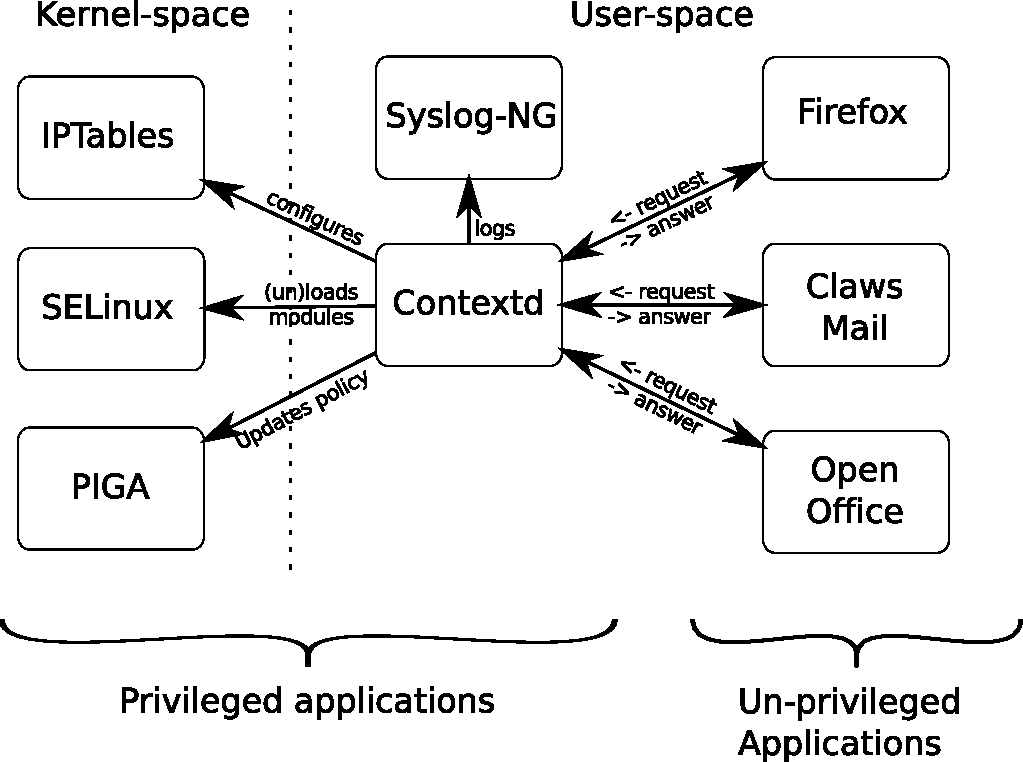
\includegraphics[width=10.5cm]{figures/architecture.pdf}
			\end{frame}

		\subsection*{Capturing the user's actions}
			\begin{frame}[fragile]
				\begin{block}{Plugin's authentication}
				\end{block}
				\vspace{0.5cm}
				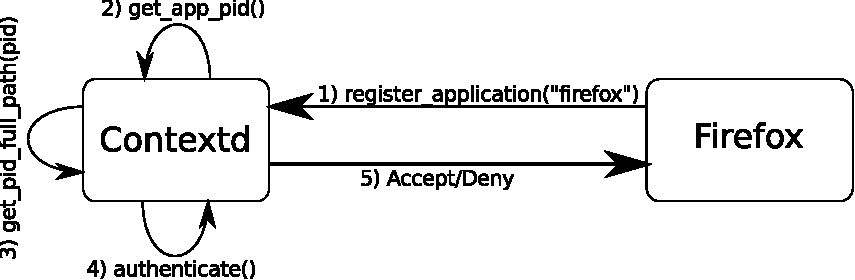
\includegraphics[width=10.5cm]{figures/app_authentication.pdf}

				\begin{verbatim}
				<program name="firefox" display_name="Firefox"
					icon="" full_path="/usr/bin/firefox" />
				\end{verbatim}
			\end{frame}

			\begin{frame}[fragile]
				\begin{block}{Plugin's communication}
				\end{block}
				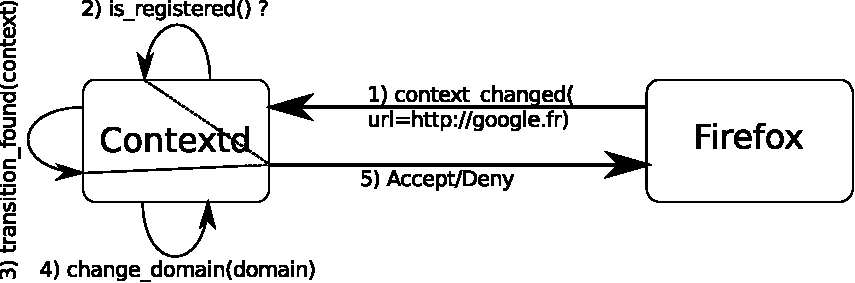
\includegraphics[width=10.5cm]{figures/app_contextchanged.pdf}

				\begin{verbatim}
					<xmlContext>
						<parameter name="url" value="http://www.google.fr" />
						<parameter name="protocol" value="http" />
						<parameter name="domain" value="www.google.fr" />
						<parameter name="port" value="80" />
						<parameter name="path" value="/" />
					</xmlContext>
				\end{verbatim}
			\end{frame}

		\subsection*{The security model}
			\begin{frame}
				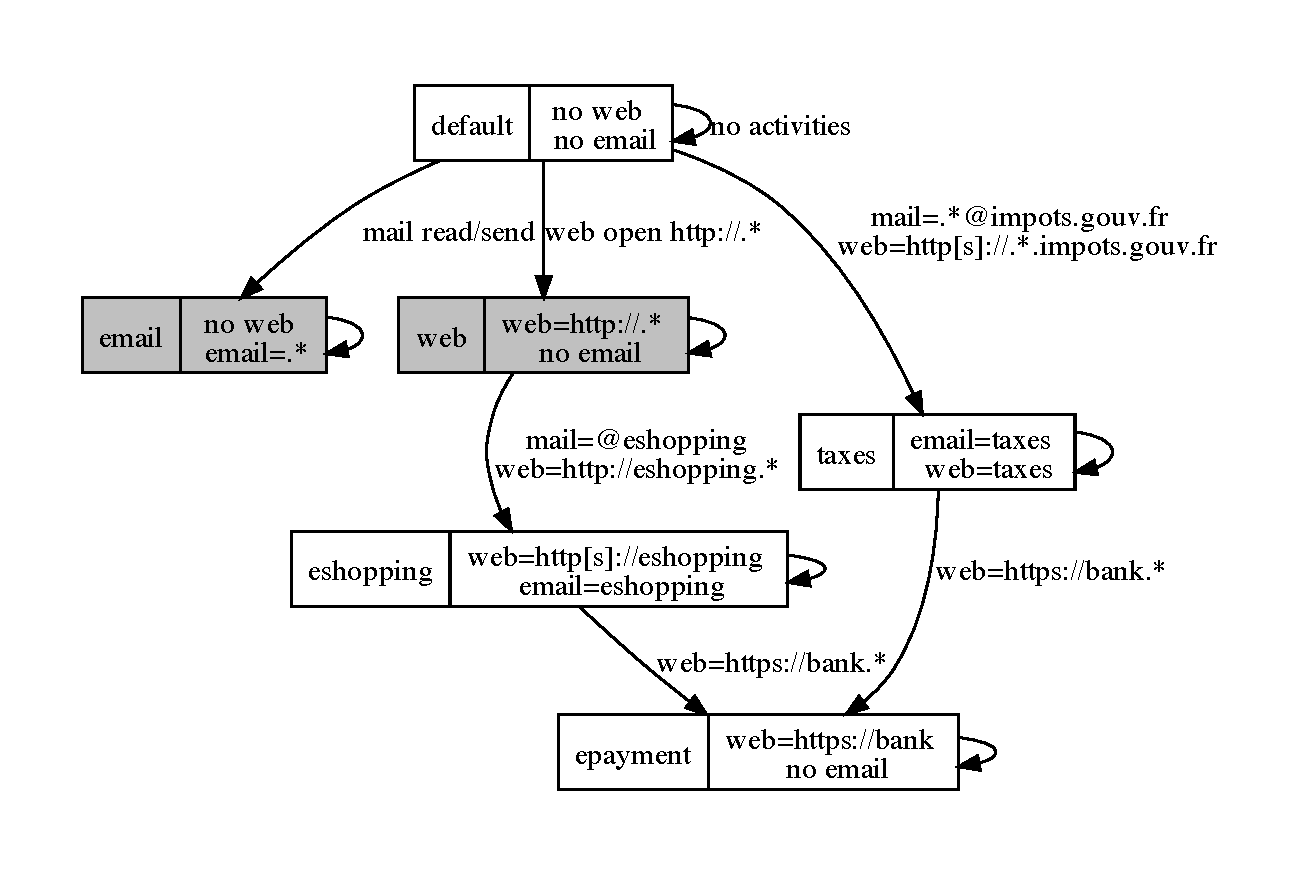
\includegraphics[width=10.5cm]{figures/transitions.pdf}
			\end{frame}

			\begin{frame}[fragile]
				\begin{block}{Domains}
					\begin{verbatim}
						<domain name="mail" display_name="E-Mail"
						icon="/usr/share/icons/evolution.png"/>
						<domain name="taxes" display_name="Taxes"
						icon="/usr/share/icons/money_coin.png"/>
					\end{verbatim}
				\end{block}

				\begin{block}{Transitions}
					\begin{verbatim}
						<rule app_name="firefox" transit_from="mail" 
							transit_to="taxes" prompt="false" notify="false">
							<host>www\.impots\.gouv\.fr</host>
							<path>.*</path>
							<protocol>(http|https)</protocol>
						</rule>
					\end{verbatim}
				\end{block}
			\end{frame}

		\subsection*{Gluing the security components}
			\begin{frame}
				\begin{block}{The internal architecture}
					Contextd's internal architecture is:
					\begin{itemize}
						\item plugin-based (each plugin having a separate configuration file and being staticly linked)
						\item event-driven
					\end{itemize}
				\end{block}
			\end{frame}

	\section{Experimentation}
		% Je montre ici notre exemple, comme dans le papier et je le commente
		% Rajout de captures d'écrans commentées ou d'une vidéo

		\subsection*{ANR's security contest}
			\begin{frame}
				The French research agency(ANR) is currently running a security contest that we decided to take part in with PIGA-OS.
				\begin{block}{ANR's security contest}
					Rules are to create a secure operating system for users to :
					\begin{itemize}
						\item Browse the internet
						\item Read e-mails
						\item Pay taxes online
						\item use e-shopping websites
					\end{itemize}
				\end{block}
			\end{frame}

		\subsection*{PIGA-OS}
			
			\begin{frame}
				\begin{block}{PIGA-OS's major components}
					\begin{itemize}
						\item Gentoo hardened: Linux distribution
						\item IPTables: Linux's default firewall
						\item Syslog-NG: Logger. For auditability purpose
						\item SELinux: Low-level, label-based MAC.
						\item PIGA: Our high-level MAC system to enforce security properties
						\item Contextd: Change the system's domain according to the user's activity and to coordinate the other components
					\end{itemize}
				\end{block}
			\end{frame}

		\subsection*{PIGA-OS Transition Graph}
			\begin{frame}
				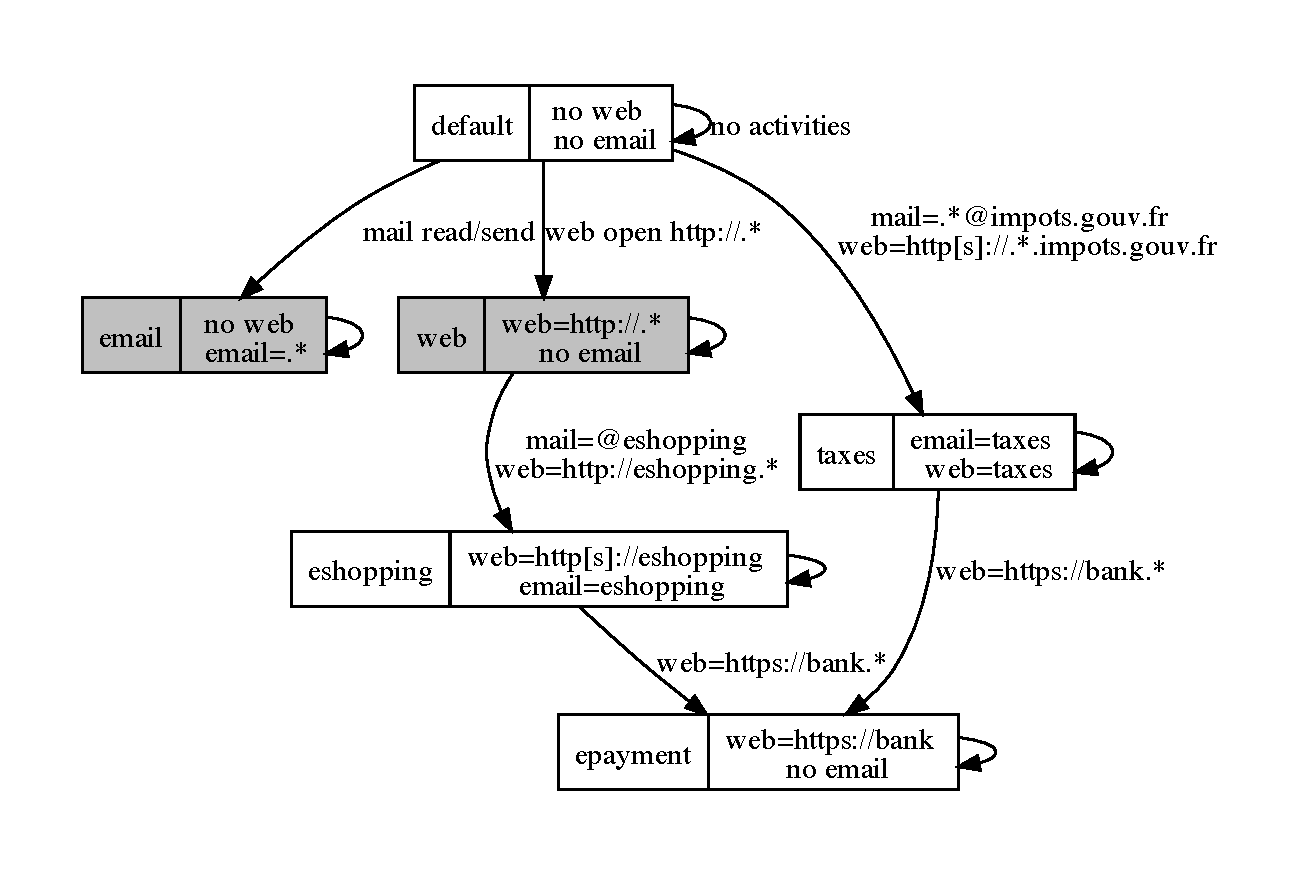
\includegraphics[width=10.5cm]{figures/transitions.pdf}
			\end{frame}

		\subsection*{PIGA-OS Screenshots}
			\begin{frame}
				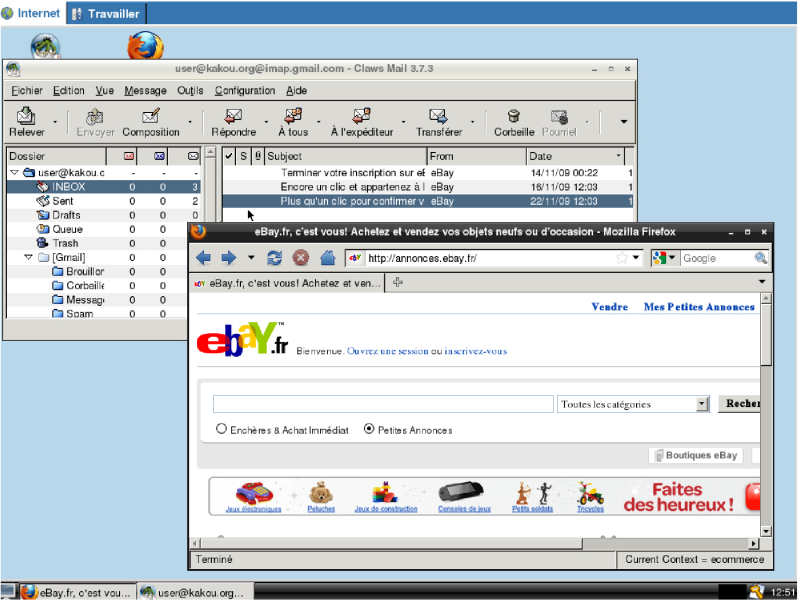
\includegraphics[width=7cm]{figures/piga-os.png}
				\hspace{0.3cm}
				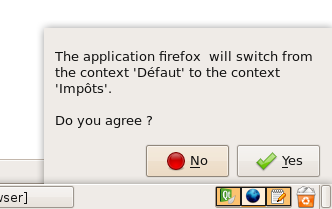
\includegraphics[width=3.2cm]{figures/contextnotifypopup.png}
			\end{frame}

			\begin{frame}
				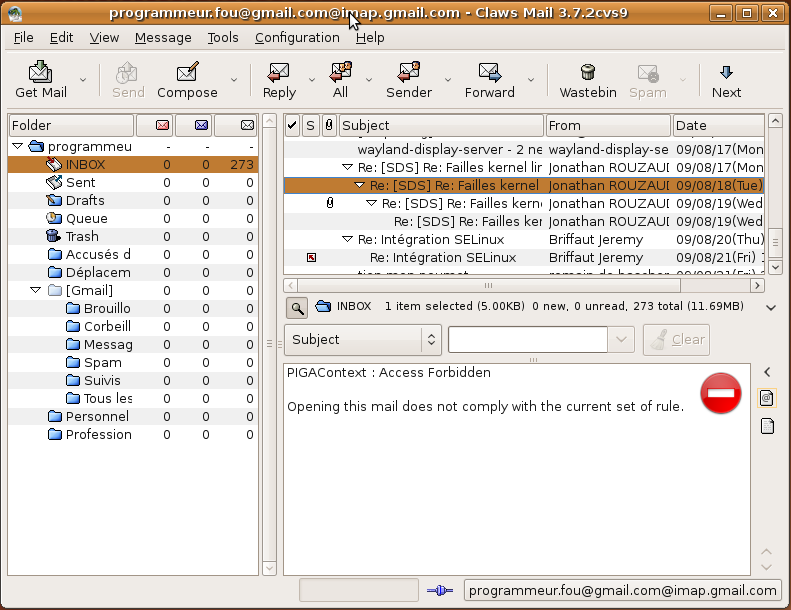
\includegraphics[width=5.1cm]{figures/clawsmail.png}
				\hspace{0.3cm}
				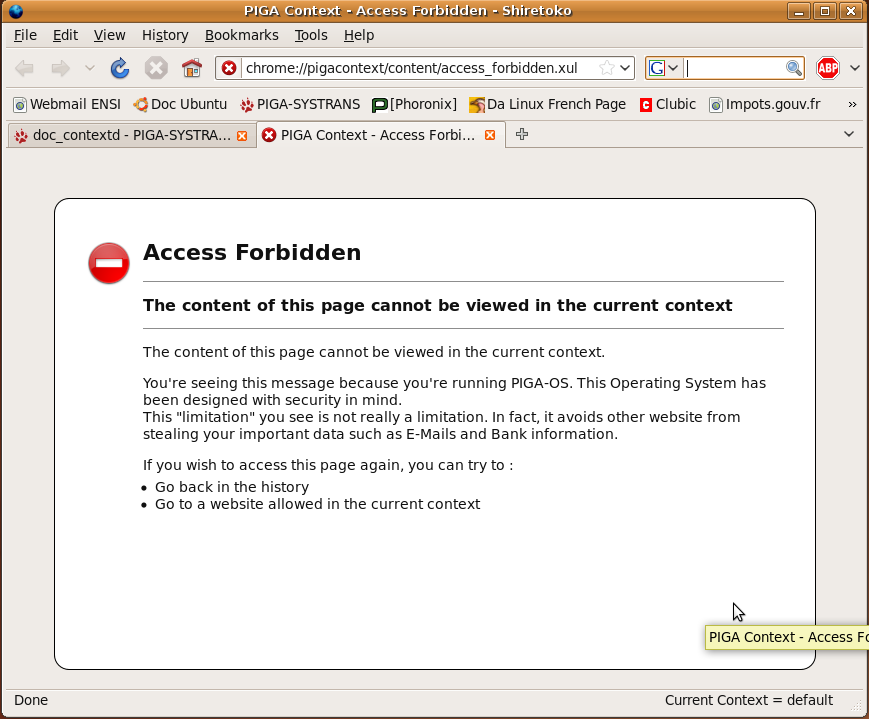
\includegraphics[width=5.1cm]{figures/firefox.png}
			\end{frame}


	\section{Conclusion}
		% En quoi c'est mieux, en quoi ça respecte ce qu'on disait en intro
		
			\begin{frame}
				\begin{block}{PIGA-OS}
					\begin{itemize}
						\item has won the ANR security contest before its end
						\item has proved better than competitors' multiple-VM-based solutions
						\item can be secure, lightweight and easy-to-use at the same time
						\item will soon be comercialized by Boken
					\end{itemize}
				\end{block}
			\end{frame}

\end{document}